\chapter{Wizja aplikacji}

\section{Wymagania funkcjonalne}
Tworzenie aplikacji należało zacząć od nakreślenia zakresu funkcjonalności, które aplikacja będzie udostępniać użytkownikom. Podstawowym zadaniem, jakie powinna spełniać jest możliwość przeprowadzania eksperymentów przy pomocy systemu GDT. Kolejnym ważnym aspektem jest wariant zarządzania, wyświetlania, udostępniania oraz edycji poszczególnych eksperymentów. Każdy z użytkowników powinien widzieć poszczególne doświadczenia, które zostały ukończone, są w trakcie lub czekają w kolejce do obliczenia. Aplikacja powinna również przede wszystkim w przejrzysty sposób wyświetlać wyniki doświadczenia w postaci wygenerowanego drzewa decyzyjnego i poszczególnych statystyk. Podczas uruchomienia nowego zadania do obliczenia, użytkownikowi zostanie wyświetlony pasek postępu oraz oszacowana długość trwania całego zadania, przy czym w dowolnym momencie będzie mógł anulować polecenie.  Wraz z możliwością tworzenia eksperymentu nie odłącznym elementem będzie funkcjonalność zarządzania plikami wejściowymi oraz wyjściowymi. Dla użytkowników początkujących zostanie przedstawiona opcja tworzenia podstawowych plików konfiguracyjnych, bez wgłębiania się w bardziej zaawansowane parametry eksperymentu. Dostęp do całej platformy wymaga założenia konta użytkownika. Natomiast możliwość rejestracji oraz logowania będzie ogólnodostępna.

System kont użytkowników powinien wyróżniać różne role, które definiowałyby dostęp do poszczególnych funkcjonalności aplikacji. Zarządzanie tymi uprawnieniami będzie się odbywać poprzez panel administratora. Administrator aplikacji dodatkowo może modyfikować oraz usuwać konta użytkowników. Co więcej z interfejsu admina będzie istniała możliwość edycji rekordów z bazy danych oraz edycja uprawnień do poszczególnych eksperymentów. 

Biorąc pod uwagę perspektywę udostępniania przez użytkownika doświadczeń innemu użytkownikowi, ważnym aspektem będzie umożliwienie ograniczenia części akcji wykonywanych na eksperymencie. Aplikacja nie pozwoli na zablokowanie wyświetlania wraz ze statystykami. Natomiast reszta funkcjonalności możliwych do wykonania na doświadczeniu, takich jak uruchamianie, kopiowanie, edycja, usuwanie czy też pobieranie plików wejściowych lub wyjściowych może zostać ograniczona. Użytkownik posiadający udostępniony eksperyment z pewnymi ograniczeniami, może udostępnić go dalej jeśli posiada nadane prawa do udostępniania. Przy czym nie może rozszerzyć uprawnień uprzednio zablokowanych.


\begin{figure}[htb]
\centering
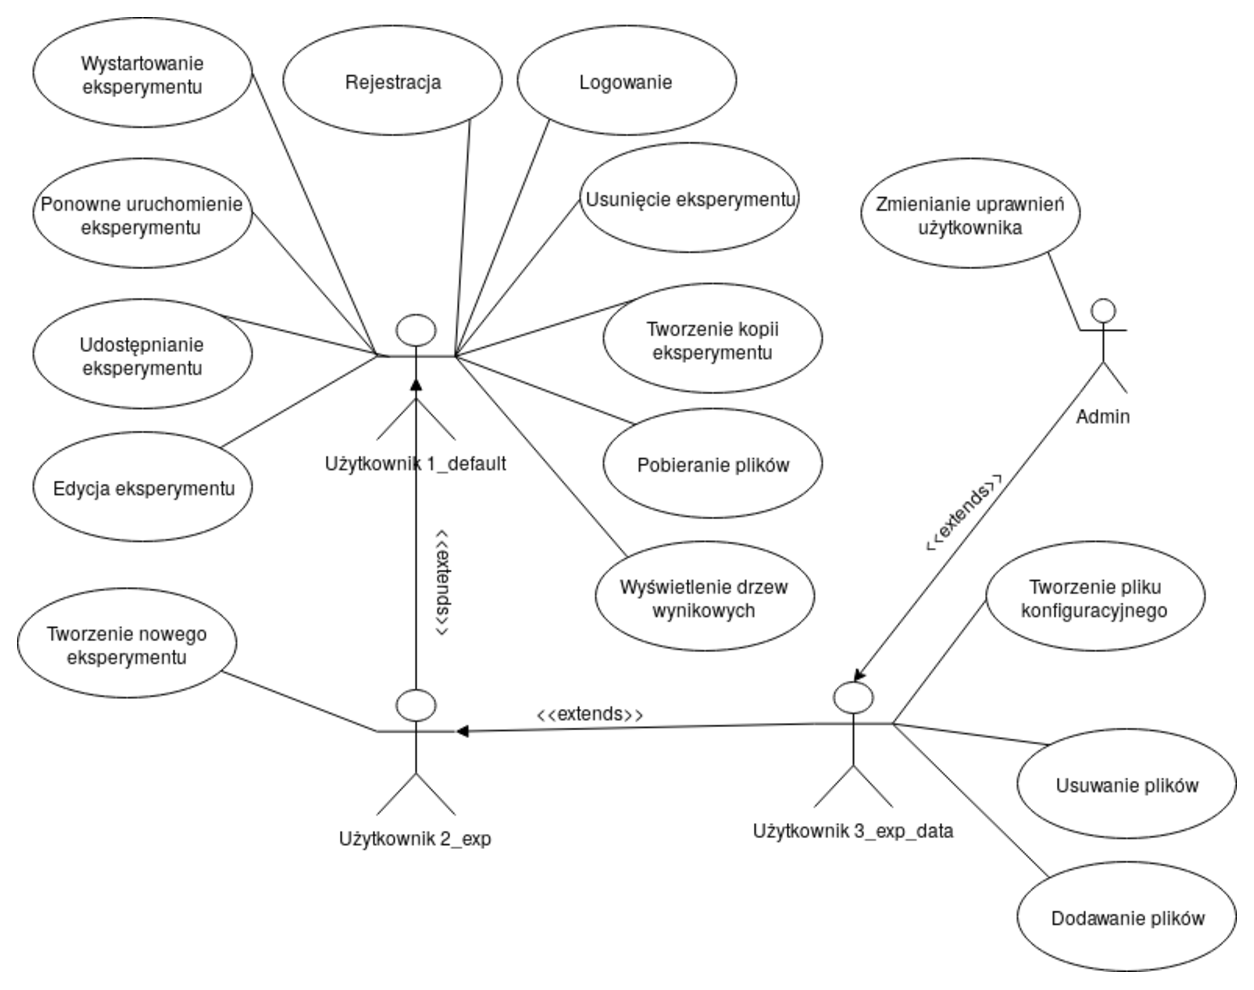
\includegraphics[width=11cm]{grafika/diagram_przypadkow_uzycia.eps}
\caption{Diagram przypadków użycia, źródło: opracowanie własne}
\label{rys1_diagram_przypadkow}
\end{figure}

\begin{figure}[htb]
	\centering
	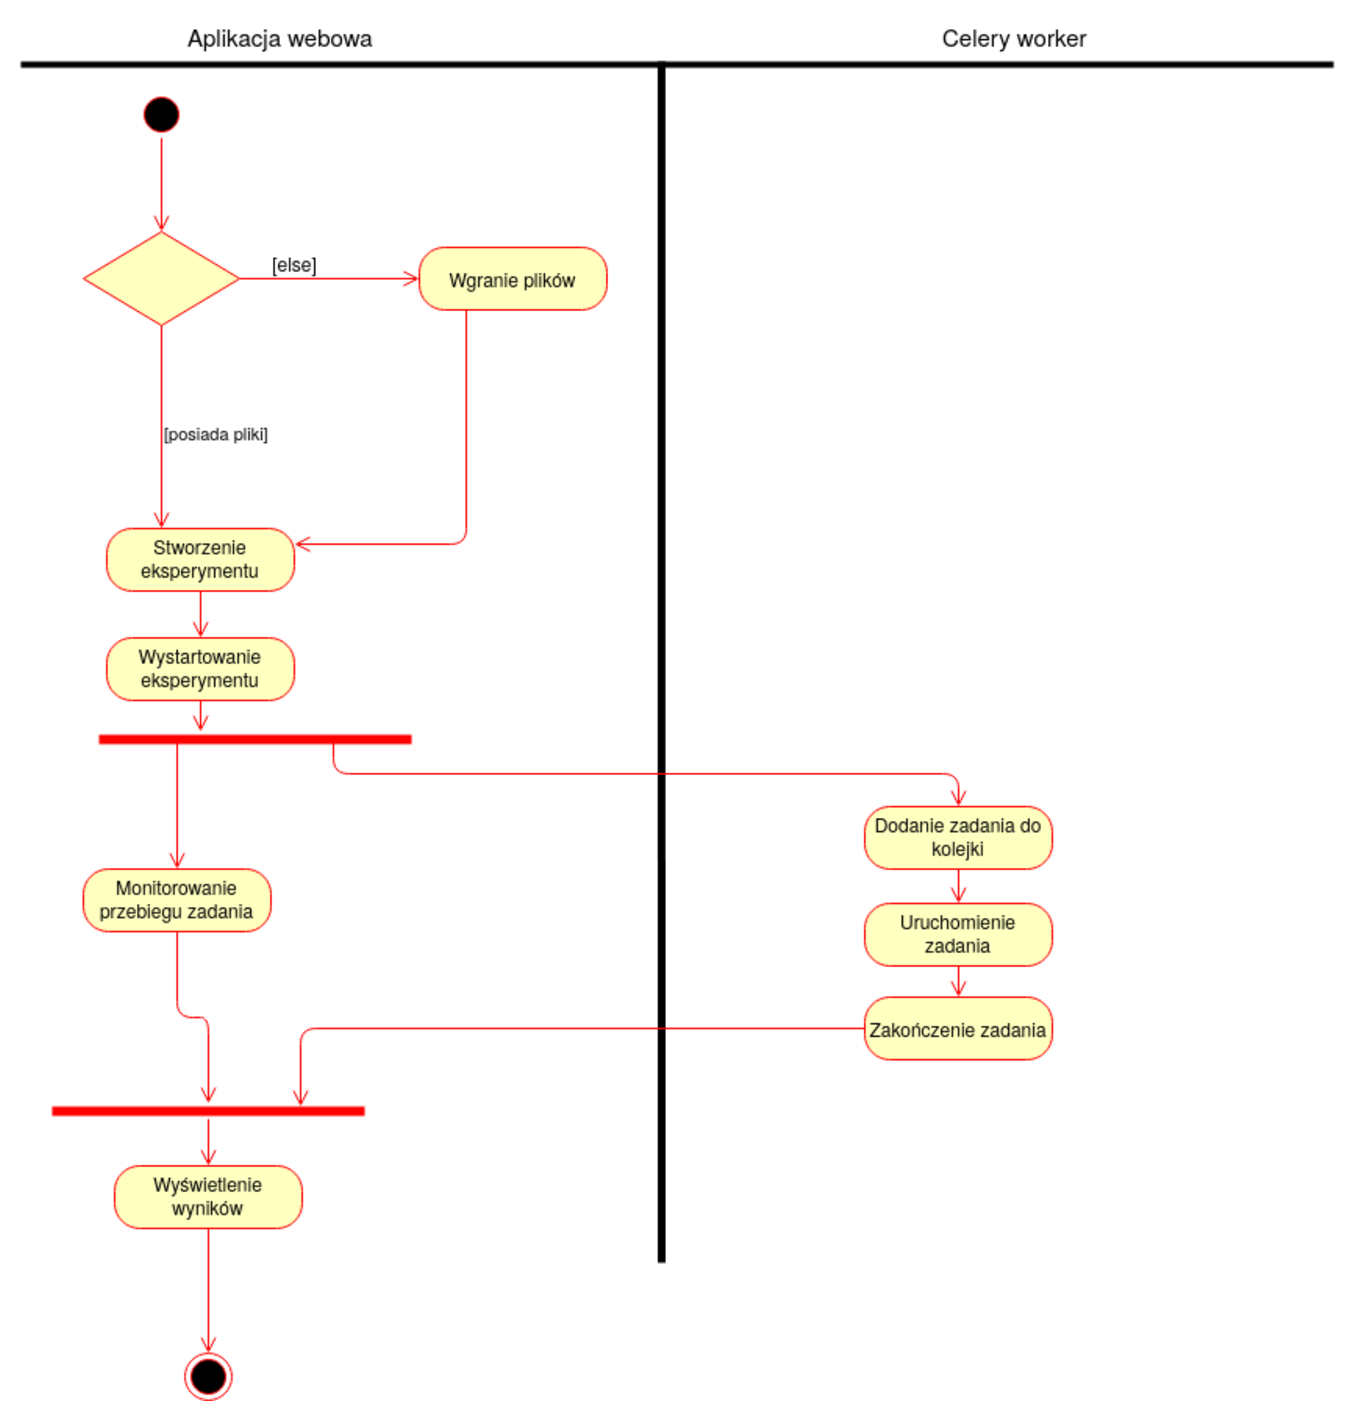
\includegraphics[width=11cm]{grafika/diagram_przebiegu_tworzenia_eksperymentu.eps}
	\caption{Diagram czynności tworzenia i uruchomiania eksperymentu, źródło: opracowanie własne}
	\label{rys2_diagram_czynności}
\end{figure}

Na rysunku \ref{rys1_diagram_przypadkow} przedstawiono wszystkie funkcjonalności w postaci diagramu przypadków użycia. W aplikacji zostały wyszczególnione trzy role dostępne do uzyskania dla każdego użytkownika oraz rola administratora całego systemu. Wszystkie przypadki użycia oprócz logowania i rejestracji są dostępne tylko dla użytkowników zalogowanych. Każdy nowy użytkownik musi założyć konto, aby mieć dostęp do aplikacji. Nowo powstałe konta otrzymują uprawnienia na domyślnym poziomie \enquote{1\_default}, a wyższe poziomy uprawnień mogą zostać nadane przez administratora. Kolejne role rozszerzają możliwości użytkownika pod względem ilości akcji do wykonania. Poziom \enquote{2\_exp} pozwala na tworzenie nowych eksperymentów, przy czym tylko najwyższy poziom uprawnień \enquote{3\_exp\_data}  może autoryzować do wgrywania plików do aplikacji. Przebieg czynności związanych ze stworzeniem nowego eksperymentu oraz wyświetleniem wyników został przedstawiony na Rys. \ref{rys2_diagram_czynności}. 



Opis przypadku użycia \enquote{Tworzenie nowego eksperymentu}:
\begin{enumerate}
\item  Aktor
	\begin{itemize}
		\item Użytkownik. 
	\end{itemize}
\item Warunki początkowe
	\begin{itemize}
		\item Aktor jest zalogowany oraz posiada uprawnienia przynajmniej na poziomie \enquote{2\_exp}.
	\end{itemize}
\item Zdarzenie inicjujące
	\begin{itemize}
		\item Naciśnięcie przycisku \enquote{New experiment} nad listą wszystkich eksperymentów użytkownika.
	\end{itemize}
\item Przebieg w krokach
	\begin{itemize}
		\item Aplikacja przechodzi do formularza tworzenia nowego eksperymentu,
		\item Użytkownik wypełnia i zatwierdza formularz.
	\end{itemize}
\item Przebiegi alternatywne
	\begin{itemize}
		\item  Użytkownik nie uzupełnia wszystkich pól formularza, aplikacja wyświetla powiadomienie o pustych polach.
	\end{itemize}
\item Sytuacje wyjątkowe
	\begin{itemize}
		\item  Użytkownik nie posiada żadnych plików wgranych do aplikacji. Powoduje to, że pola formularza zawierające pliki są puste. Uniemożliwia to stworzenie nowego eksperymentu, a aplikacja wyświetla powiadomienie o pustych polach przy podjętej próbie zatwierdzenia.
	\end{itemize}
\item Warunki końcowe
	\begin{itemize}
		\item  System przekierowuje użytkownika do listy z eksperymentami, a na liście znajduje się nowo utworzony eksperyment.
	\end{itemize}
\item Zależności czasowe
	\begin{itemize}
		\item  Częstotliwość wykonywania: Około 20 razy dziennie na każdego użytkownika,
		\item Typowy czas realizacji: 8 sekund.
	\end{itemize}
\end{enumerate}

Opis przypadku użycia \enquote{Wystartowanie eksperymentu}:
\begin{enumerate}
	\item  Aktor
	\begin{itemize}
		\item Użytkownik. 
	\end{itemize}
	\item Warunki początkowe
	\begin{itemize}
		\item Aktor jest zalogowany oraz posiada stworzony eksperyment.
	\end{itemize}
	\item Zdarzenie inicjujące
	\begin{itemize}
		\item Naciśnięcie przycisku \enquote{Show} w liście eksperymentów na elemencie, którego status to \enquote{Created}.
	\end{itemize}
	\item Przebieg w krokach
	\begin{itemize}
		\item Aplikacja przechodzi do podglądu szczegółów wybranego eksperymentu,
		\item Użytkownik klika przycisk \enquote{Start} znajdujący się na pasku możliwych czynności,
		\item Aplikacja przekierowuje użytkownika do listy eksperymentów.
	\end{itemize}
	\item Przebiegi alternatywne
	\begin{itemize}
		\item  Po wystartowaniu eksperymentu nastąpił błąd i jest to sygnalizowane zmianą statusu na \enquote{Error}, a w szczegółach eksperymentu można podejrzeć wiadomość z błędem.
	\end{itemize}
	\item Sytuacje wyjątkowe
	\begin{itemize}
		\item  Użytkownikowi nie posiada prawd do wystartowania konkretnego eksperymentu i w panelu akcji nie wyświetla się przycisk \enquote{Start}.
	\end{itemize}
	\item Warunki końcowe
	\begin{itemize}
		\item  Eksperyment zmienił swój status na \enquote{In queue} lub \enquote{Running}, a po przejściu do szczegółów wyświetla się pasek postępu oraz szacowany czas oczekiwania na zakończenie.
	\end{itemize}
	\item Zależności czasowe
	\begin{itemize}
		\item Częstotliwość wykonywania: Około 20 razy dziennie na każdego użytkownika,
		\item Typowy czas realizacji: 8 sekund.
	\end{itemize}
\end{enumerate}

Opis przypadku użycia \enquote{Wyświetlenie drzewa wynikowego}:
\begin{enumerate}
	\item  Aktor
	\begin{itemize}
		\item Użytkownik. 
	\end{itemize}
	\item Warunki początkowe
	\begin{itemize}
		\item Aktor jest zalogowany oraz posiada ukończony eksperyment.
	\end{itemize}
	\item Zdarzenie inicjujące
	\begin{itemize}
		\item Naciśnięcie przycisku \enquote{Show} w liście eksperymentów na elemencie, którego status to \enquote{Finished}.
	\end{itemize}
	\item Przebieg w krokach
	\begin{itemize}
		\item Aplikacja przechodzi do podglądu szczegółów wybranego eksperymentu, a na samym dole karty wyświetlają się linki do drzew decyzyjnych,
		\item Użytkownik klika w link do drzewa decyzyjnego.
	\end{itemize}
	\item Przebiegi alternatywne
	\begin{itemize}
		\item  Brak.
	\end{itemize}
	\item Sytuacje wyjątkowe
	\begin{itemize}
		\item  Brak.
	\end{itemize}
	\item Warunki końcowe
	\begin{itemize}
	\item  Aplikacja wyświetliła drzewo decyzyjne wraz ze statystykami.
	\end{itemize}
	\item Zależności czasowe
	\begin{itemize}
		\item Częstotliwość wykonywania: Około 30 razy dziennie na każdego użytkownika,
		\item Typowy czas realizacji: 10 sekund.
	\end{itemize}
\end{enumerate}

\section{Wymagania niefunkcjonalne}
Projekt aplikacji zostanie podzielony na dwa oddzielne komponenty jeden odpowiadający za stronę internetową, drugi natomiast za kolejkowanie i uruchamianie zadań w systemie GDT. Kompletne oprogramowanie pozwala na zarządzanie całością aplikacji w dość przejrzysty sposób. Poszczególne elementy strony serwerowej powinny być odporne na błędy, umożliwiać łatwy mechanizm wdrożenia oraz restartu modułów w przypadku takiej potrzeby. Zostanie to zapewnione poprzez konteneryzacje aplikacji. Zależności pomiędzy konkretnymi kontenerami utworzonymi przy pomocy oprogramowania Docker zostały przedstawione na Rys. \ref{rys3_architektura_systemu}. Dzięki takiemu rozwiązaniu wdrożenie aplikacji, czy też zmiana któregoś z komponentów na przykład serwera bazy danych, jest możliwa w sposób natychmiastowy i mało inwazyjny. Jedyną rzeczą niezbędna na serwerze, aby uruchomić aplikacje jest platforma Docker.    

\begin{figure}[htb]
	\centering
	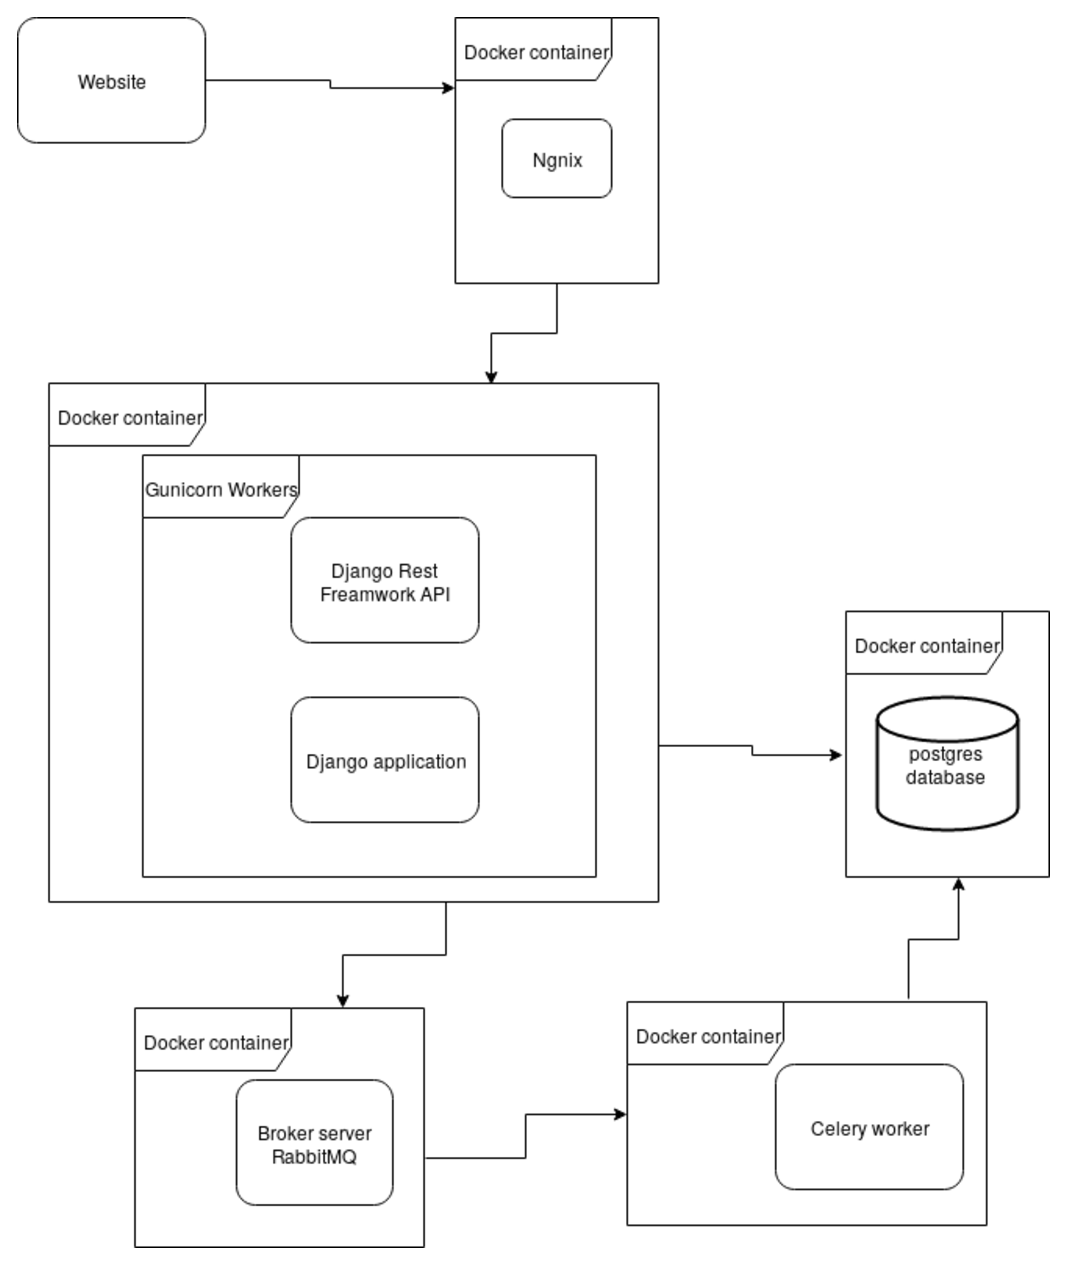
\includegraphics[width=11cm]{grafika/architektura_systemu.eps}
	\caption{Architektura systemu, źródło: opracowanie własne}
	\label{rys3_architektura_systemu}
\end{figure}

\section{Wykorzystane technologie}
Aplikacja zostanie zaimplementowana z użyciem języka programowania Python, który zyskuję coraz większą popularność wśród programistów. Charakteryzuje się on łatwym progiem wejścia oraz wspieraniem kilku różnych paradygmatów programowania takich jak programowanie funkcyjne, proceduralne i obiektowe \cite{book_3}. Po stronie serwera będzie wystawione API w architekturze REST (\textit{Representational State Transfer}) z wykorzystaniem Django oraz Django REST Framework. Natomiast interfejs graficzny strony będzie zaprojektowany przy pomocy JavaScriptu oraz biblioteki ReactJS.

Jedną z najważniejszych cech języka Python jest interpretowalność kodu źródłowego zamiast jego kompilacja \cite{misc_python}. Umożliwia on pisanie zarówno skryptów jak i zaawansowane programy. Kolejnym jego atrybutem jest dynamiczne typowanie czyli tak zwany \textit{duck typing}. Określa to sposób przypisywania typów do wartości przechowywanych w zmiennych. Typy te są określane dynamicznie podczas działania programu, w odróżnieniu od typowania statycznego, gdy wartości poszczególnych zmiennych muszą być jasno podane przed procesem kompilacji. Takie podejście do przypisywania rodzajów na pewno przyśpiesza pracę, ale wiążę się z pewnymi wadami. W trakcie implementacji, programista musi sam pamiętać jaki typ w danym momencie ma zmienna. Z pomocą przychodzi biblioteka wbudowana w język o nazwie Typing. Umożliwia ona w prosty sposób wprowadzenie namiastki typowania statycznego w postaci sprawdzania i podpowiedzi.

Do implementacji części biznesowej aplikacji zostanie wykorzystany framework Django, który jest jednym z najbardziej popularnych rozwiązań webowych w języku Python. Charakteryzuje się on dużą szybkością implementacji oraz jasnym podziałem aplikacji na konkretne komponenty. Zarazem narzuca on pewną strukturę projektu, która zapewnia czystość kodu oraz możliwość ponownego używania wcześniej opracowanych modułów \cite{misc_django}. Społeczność zebrana wokół tej platformy, czynnie rozwija nowe rozwiązania, które są udostępniane dla szerszego grona odbiorców. Dzięki temu istnieje łatwy dostęp do wysokiej jakości modułów bezpieczeństwa, czy też wsparcie techniczne przy występujących problemach. Kolejnym argumentem, który przemawiał za wybraniem tej technologi był wbudowany panel administratora, dostarczany wraz z całą platformą. Po konfiguracji umożliwia on nie tylko zarządzanie użytkownikami, ale także edycje rekordów w bazie danych. 

W celu wystawienia REST API(\textit{Representational State Transfer Application Programming Interface}) dla interfejsu graficznego został użyty Django REST Framework (\textit{DRF}), który wraz z podstawową wersją Django stanowi trzon aplikacji. DRF jest narzędziem używanym oraz rozwijanym przez takie rozpoznawalne marki jak  Mozilla, Red Hat, Heroku \cite{misc_django_rest}. Świadczy to nie tylko o popularności tego rozwiązania, ale też o jakości jego wykonania. Cały framework skupia się na wystawieniu dla programisty zestawu narzędzi do budowy interfejsu restowego. W skład takiej paczki wchodzą serializatory(\textit{serializers}), widoki(\textit{views}), rutery(\textit{router}) oraz wiele innych pomocniczych obiektów. Komunikacja z takim interfejsem programistycznym odbywa się za pomocą metod protokołu http. Kolejność kroków pracy API możemy określić w następujący sposób:
\begin{enumerate}
	\item Klient tworzy zapytanie i uzupełnia je o potrzebne dane, 
	\item Następnie następuje wysłanie zapytania pod konkretny adres,
	\item Serwer przetwarza żądanie klienta oraz wysyła odpowiedź,
	\item Klient otrzymuje rezultat.
\end{enumerate}

Do zapisu informacji związanych z działaniem aplikacji zostanie wykorzystana relacyjna baza danych PostgreSQL. Jest to rozwiązanie pod licencją \textit{Open Source} i szeroko stosowane również z aplikacjami opartymi o technologie Django. Bazę można w łatwy sposób podpiąć pod panel administratora, ale także uzyskać dostęp z poziomu kodu aplikacji. W bazie danych będą zapisywane konta użytkowników oraz informacje o stworzonych eksperymentach wraz ze ścieżkami do plików. 

Biblioteka ReactJS łącznie z JavaScriptem pozwoli na zaimplementowanie funkcjonalnego interfejsu graficznego strony internetowej. Zapewnia ona pewną strukturę projektu, która oferuje czystość kodu, czytelność oraz wygodę użytkowania. Pozwala na wstawianie wstawek kodu hmtl do kodu JavaScrioptowego za pośrednictwem języka JSX. Początkowo bibliotek została stworzona dla potrzeb wewnętrznych firmy Facebook, ale z czasem została udostępniona innym twórcom \cite{misc_react}. Programiści na całym świecie tak docenili te rozwiązanie, że ReactJS jest aktualnie wykorzystywany przez wielkie korporacje takie jak Netflix czy Uber, a sam projekt jest czwartym najpopularniejszym repozytorium na GitHub \cite{misc_react_pop}. W celu połączenia interfejsu graficznego z logiką biznesową wystawioną za pomocą REST API została wykorzystana biblioteka Axios \cite{misc_axios}. Cechuje się implementacją klienta http działająca po stronie strony internetowej. Umożliwia ona budowę zapytań http oraz ich realizację. Aktualnie jest to najpopularniejsze rozwiązanie w języku JavaScript. 

W celu uzyskania pełnej asynchroniczności podczas uruchamiania eksperymentów w systemie GDT, do obsługi kolejki zadań zostanie wykorzystana biblioteka Celery \cite{misc_celery}. Takie rozwiązanie jest łatwe w integracji z innymi platformami programistycznymi. Głównym założeniem działania tej biblioteki polega na stworzeniu kolejki z zadaniami, które następnie zostaną przypisane i wykonane przez wolnego robotnika. Liczba robotników działających w aplikacji może zostać określona jako jeden z parametrów uruchomienia. Komunikacja pomiędzy Celery, a aplikacją w technologi Django odbywa się przy pomocy brokera wiadomości (\textit{message broker}), który odpowiada za przesył informacji pomiędzy dwoma komponentami. Przykładem takiego oprogramowania może być broker RabbitMQ i on zostanie wykorzystany podczas implementacji aplikacji dyplomowej \cite{misc_rabbit}. Oprogramowanie do wymiany wiadomości od Pivotal Software osiąga bardzo dobre wyniki wydajnościowe w porównaniu z produktami konkurencyjnymi.

Gunicorn jest serwerem http aplikacji Django, umożliwiającym zdefiniowanie liczby robotników realizujących zapytania. Jego głównym założeniem jest realizacja wszystkiego co się dzieje pomiędzy serwerem, a aplikacją webową. Dodatkowym atutem jest minimalna ilość zasobów, które zużywa oraz duża szybkość działania \cite{misc_gunicorn}. W projekcie strony internetowej zostanie wykorzystany zaraz obok serwera www o nazwie Nginx pełniącego rolę pośrednika zapytań. Serwer www posłuży do przekierowania przychodzących pod adres domeny \enquote{decisiontree.pl} żądań prosto do aplikacji działającej pod serwerem Gunicorn.

Jedną z najważniejszych części całej architektury jest konteneryzacja poszczególnych elementów. W tym celu zostaną wykorzystane kontenery stworzone przy pomocy platformy Docker. Jest to oprogramowanie umożliwiający łatwą wirtualizacje oraz podział projektu na oddzielne komponenty \cite{misc_docker}. Stosując takie rozwiązanie w dowolnej chwili można podmieniać ze sobą kontenery aplikacji, zmieniając dynamicznie ich wersje oraz łatwo restartować tylko te elementy, które tego wymagają. Cały system zostanie podzielony na pięć pracujących obok siebie instancji tworzących wspólnie całość. Podział ten jest przedstawiony na Rys. \ref{rys3_architektura_systemu}.


 
 





